\documentclass[a4paper]{article}
\usepackage[spanish]{babel}
\title{Taller 1}

\usepackage[utf8]{inputenc}
\usepackage{caratula}
\usepackage{graphicx}
\usepackage{color}
\usepackage{listings}
\usepackage{float}

\setlength{\leftmargin}{2cm}
\setlength{\rightmargin}{2cm}
\setlength{\oddsidemargin}{-1cm}
\setlength{\evensidemargin}{-1cm}
\setlength{\topmargin}{-1cm}
\setlength{\textwidth}{18cm}
\setlength{\textheight}{25cm}

\usepackage{fancyhdr}
\pagestyle{fancy}
\fancyhf{}
\fancyhead [LO,LE]{\scriptsize Trabajo Práctico N$^{\circ}$1}
\fancyhead [RO,RE]{\scriptsize Mancuso, Mataloni, Tolchinsky}
\fancyfoot[CE,CO]{\thepage}
\renewcommand{\footrulewidth}{0.4pt}

\usepackage[pdftex, bookmarks=true, colorlinks, citecolor=black, linkcolor=black]{hyperref}
\usepackage{multirow}

\begin{document}

\materia{Teoria de las comunicaciones}
\submateria{Segundo Cuatrimestre de 2012}
\titulo{Taller de Capa de Enlace}
\grupo{Taller N$^{\circ}$1}

\integrante{Mancuso, Emiliano}{597/07}{emiliano.mancuso@gmail.com}
\integrante{Mataloni, Alejandro}{706/07}{amataloni@gmail.com}
\integrante{Curtua, Matias}{453/07}{curtu_infinito73@hotmail.com}

\maketitle

\newpage

\addcontentsline{toc}{section}{Índice}
\tableofcontents

% Main project

\newpage

\section{Primera consigna}

Lo que hicimos fue implementar en \textit{Scapy} un script que, dada una dirección IP, realiza un pedido por la dirección física y recibe y muestra la respuesta en caso de ser recibida. \\

El script es el siguiente:

\begin{verbatim}
pkt = ARP(pdst=sys.argv[1], op="who-has");
response = sr1(pkt)
response.show()
\end{verbatim}


Lo interesante es ver que ocurre en algunos casos:

\begin{itemize}
\item dirección inexistente = el script se cuelga esperando la respuesta que nunca llega. 
\item dirección de la maquina de origen = el paquete ARP no se envía.
\item dirección broadcast = pregunta por la dirección por lo que pasa lo mismo que si fuera una dirección inexistente 
\item dirección de red = pregunta por la dirección por lo que pasa lo mismo que si fuera una dirección inexistente 
\end{itemize}


\section{Segunda consigna}

Implementamos un script en \textit{Scapy} para escuchar pasivamente en la red y capturar cada mensaje ARP capturado. En el mismo script cuando capturamos el mensaje leemos los datos para obtener los vendors y exibirlos por pantalla.\\

El script es el siguiente:

\begin{verbatim}
# Build the vendor dictionary
ins = open( "vendorsUtil.txt", "r" )
vendors_dict = {}
for line in ins:
    vendors_dict[line[0:8]] = line[9:-1] 
ins.close()

# Print pretty vendor
def arp_monitor_callback(pkt):
	vendor_prefix = pkt[ARP].hwsrc[0:8].upper()
	strr =  pkt[ARP].psrc + ": \t" + vendors_dict[vendor_prefix]
	print strr

if len(sys.argv) == 1:
	print "Listening for 5 seconds.."
	to = 5  # Default value
else:
	to = int(sys.argv[1]) 

sniff(prn=arp_monitor_callback, filter="arp", store=0, timeout=to)
\end{verbatim}

\newpage

\section{Tercera consigna}

Para esta parte lo que hicimos fue capturar los paquetes \textit{ARP}, y crear un grafo dirigido de IPs. Cada nodo representa una dirección IP y existe un eje entre los nodos \textit{x} e \textit{y} si y solo si se observo un request ARP con source el IP del nodo \textit{x} y target igual al IP que representa el nodo \textit{y}. Consideramos que esta es la mejor forma para extraer informacion en cuanto a la topologia de la red en cuestión, asi como también sacar datos interesantes de la misma.\\\\

\begin{figure}[H]
  \centering
  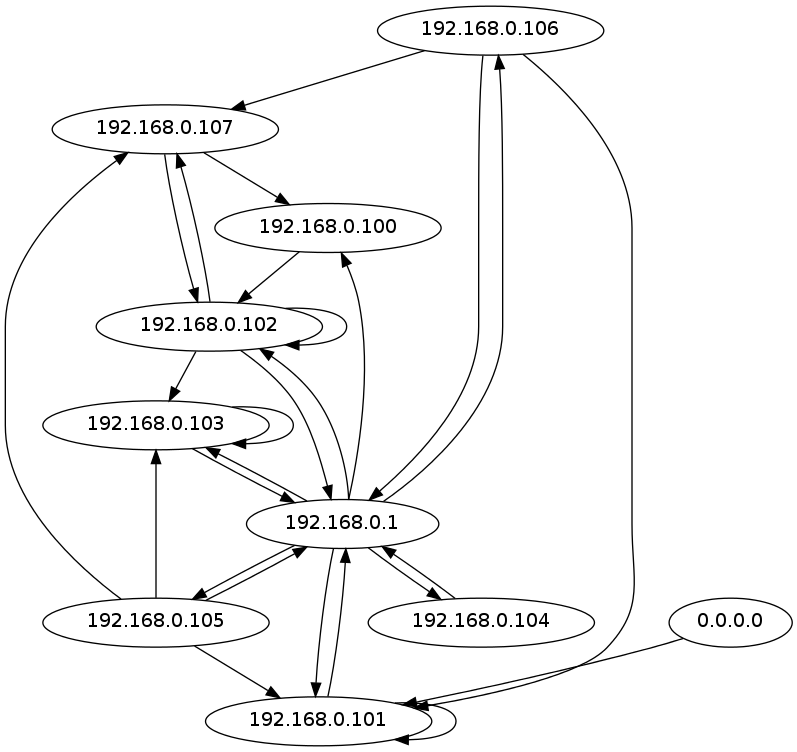
\includegraphics[scale=0.30]{graficos/arpGraph.png}
  \caption{Gráfico dirigido de los distintos request ARP observados.}
\end{figure}

 



\end{document}
